\RequirePackage[hyphens]{url}
\documentclass[sigconf]{acmart}
\raggedbottom

\usepackage{hyperref}

%\usepackage{endfloat}
%\renewcommand{\efloatseparator}{\mbox{}} % no new page between figures

\usepackage{booktabs} % For formal tables

\settopmatter{printacmref=false} % Removes citation information below abstract
\renewcommand\footnotetextcopyrightpermission[1]{} % removes footnote with conference information in first column
\pagestyle{plain} % removes running headers


\begin{document}

\title{BigchainDB: A Big Database for the Blockchain?}
\author{Timothy A. Thompson}
%\orcid{0000-0001-6574-9010}
\affiliation{%
  \institution{Indiana University Bloomington}
  \streetaddress{School of Informatics, Computing, and Engineering}
  \city{Bloomington} 
  \state{Indiana} 
  \postcode{47408}
}
\email{timathom@indiana.edu}

\begin{abstract} 
Decentralized systems such as Bitcoin, the Interplanetary File System (IPFS), and Ethereum have been designed with the intention of reengineering the architecture of online information networks, of minimizing exposure through centralized points of failure, and of creating new social models for the exchange of data---which is posited as a valuable asset in and of itself. Are these kinds of systems also able to support big data analytics and processing? If so, what stands to be gained by taking a blockchain-based approach to big data? Efforts to integrate blockchains into big data pipelines must inevitably address the tradeoff between security and scalability. BigchainDB is a new decentralized database framework that adds blockchain-based features, such as immutability and secure asset management, to traditional NoSQL distributed databases. Although it is still in the early stages of development, BigchainDB promises to make a significant contribution to the ways in which data is shared, processed, and managed at scale.
\end{abstract}

\keywords{i523, HID340, Decentralization, Databases, NoSQL, Blockchains, BigchainDB}

\maketitle

\section{Introduction}
Approaches to managing and processing big and complex data, such as the Lambda Architecture framework, have stressed the importance of treating data as an immutable asset \cite{nM15}. In this view, data should never be updated, but only appended. In systems that allow data to be deleted or updated, big data only amplifies the surface of exposure to human error, and systems that conform to the standard relational database model of incremental updates become increasingly brittle as the scale of data increases \cite{nM15}. Inadvertent deletions can trigger a cascade of data loss and system disruption that can be particularly difficult and costly to recover from. Even those who have criticized the specifics of the Lambda Architecture model (which proposes a complex internal division, within big data systems, between a batch layer and a realtime layer) agree that data immutability is an important foundation for building massively scalable platforms \cite{jK14}.

In decentralized, blockchain-based systems such as Bitcoin, immutability takes on an even more critical role. Without immutability and concomitant mechanisms such as Merkle tree hashing, it would not be possible to verify Bitcoin transactions for authenticity, nor would it be possible to maintain the ``trustless'' nature of the network---which is what allows decentralization itself to succeed \cite{aA17}. In addition to Bitcoin, the emerging decentralized data ecosystem currently comprises platforms for computation (Ethereum) and file storage (Interplanetary File System---IPFS), but database software for managing metadata about assets is still lacking. BigchainDB is a databse solution that has been designed to fill this niche \cite{bigDB16}.

\section{Distributed versus Decentralized}
Once it has been elevated to a core piece of system architecture, data immutability can become either a burden or an opportunity. The Lambda Architecture model leverages immutability within the context of an internally distributed environment, using storage solutions such as the Hadoop Distributed File System for processing on the batch layer \cite{nM15}. Distributed systems are not the same as decentralized systems, however, and the terminology itself can be misleading, as illustrated by Baran's often-reproduced work depicting the continuum between centralized and distributed networks (shown in Figure \ref{f:baran}).

\begin{figure}
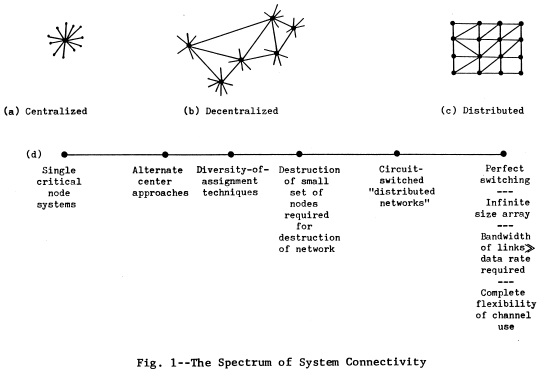
\includegraphics[width=1.0\columnwidth]{images/baran-fig1.png}
\caption{Baran's centralized--distributed network continuum \cite{pB64}}
\label{f:baran}
\end{figure}

\subsection{Tradeoffs between Security and Scalability}
Security and scalability \cite{aA17, bigDB16, bigDB17a, bigDB17b, jC17, kB16, kC16, nM15, tMAI17, tMBD16, sR16}.

Testing \ref{f:baran} testing.

\subsection{Blockchains for Big Data}

\section{BigchainDB}

\section{Conclusion}

\begin{acks}
The author would like to thank Dr. Gregor von Laszewski and the i523 teaching assistants for their support and suggestions in writing this paper.
\end{acks}

\bibliographystyle{ACM-Reference-Format}
\bibliography{report} 

\end{document}
